\documentclass[border=10pt]{standalone}
\usepackage{tikz}
\usetikzlibrary{arrows.meta, shapes, calc}

\begin{document}

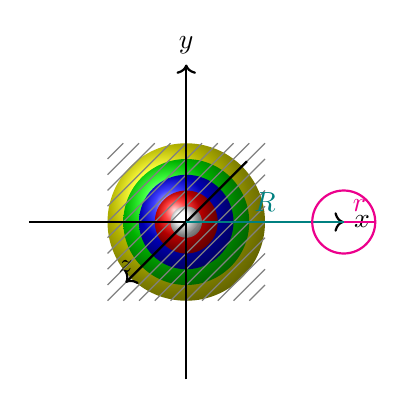
\begin{tikzpicture}[scale=2]
    % Define colors for the torus
    \definecolor{torusColor}{RGB}{255, 255, 0} % Yellow
    \definecolor{torusColor2}{RGB}{0, 255, 0} % Green
    \definecolor{torusColor3}{RGB}{0, 0, 255} % Blue
    \definecolor{torusColor4}{RGB}{255, 0, 0} % Red
    \definecolor{torusColor5}{RGB}{255, 255, 255} % White

    % Draw the torus
    \shade[ball color=torusColor] (0,0) circle (0.5);
    \shade[ball color=torusColor2] (0,0) circle (0.4);
    \shade[ball color=torusColor3] (0,0) circle (0.3);
    \shade[ball color=torusColor4] (0,0) circle (0.2);
    \shade[ball color=torusColor5] (0,0) circle (0.1);

    % Draw the grid on the torus
    \foreach \x in {-0.5, -0.4, ..., 0.5}
        \foreach \y in {-0.5, -0.4, ..., 0.5}
            \draw[gray, thin] (\x,\y) -- (\x+0.1,\y+0.1);

    % Draw the axes
    \draw[->, thick] (-1,0,0) -- (1,0,0) node[right] {$x$};
    \draw[->, thick] (0,-1,0) -- (0,1,0) node[above] {$y$};
    \draw[->, thick] (0,0,-1) -- (0,0,1) node[above] {$z$};

    % Draw the radius R
    \draw[teal, thick] (0,0,0) -- (1,0,0) node[midway, above] {$R$};

    % Draw the smaller circle
    \draw[thick, magenta] (1,0,0) circle (0.2);

    % Draw the radius r
    \draw[thick, magenta] (1,0,0) -- (1.2,0,0) node[midway, above] {$r$};

\end{tikzpicture}

\end{document}